\chapter{Applicability of the Fisher Matrix}
\label{app:fisher_valid}

\chapter{Oscillation Probabilities}
\label{app:oscillation}

\begin{figure}[h]
 \centering
 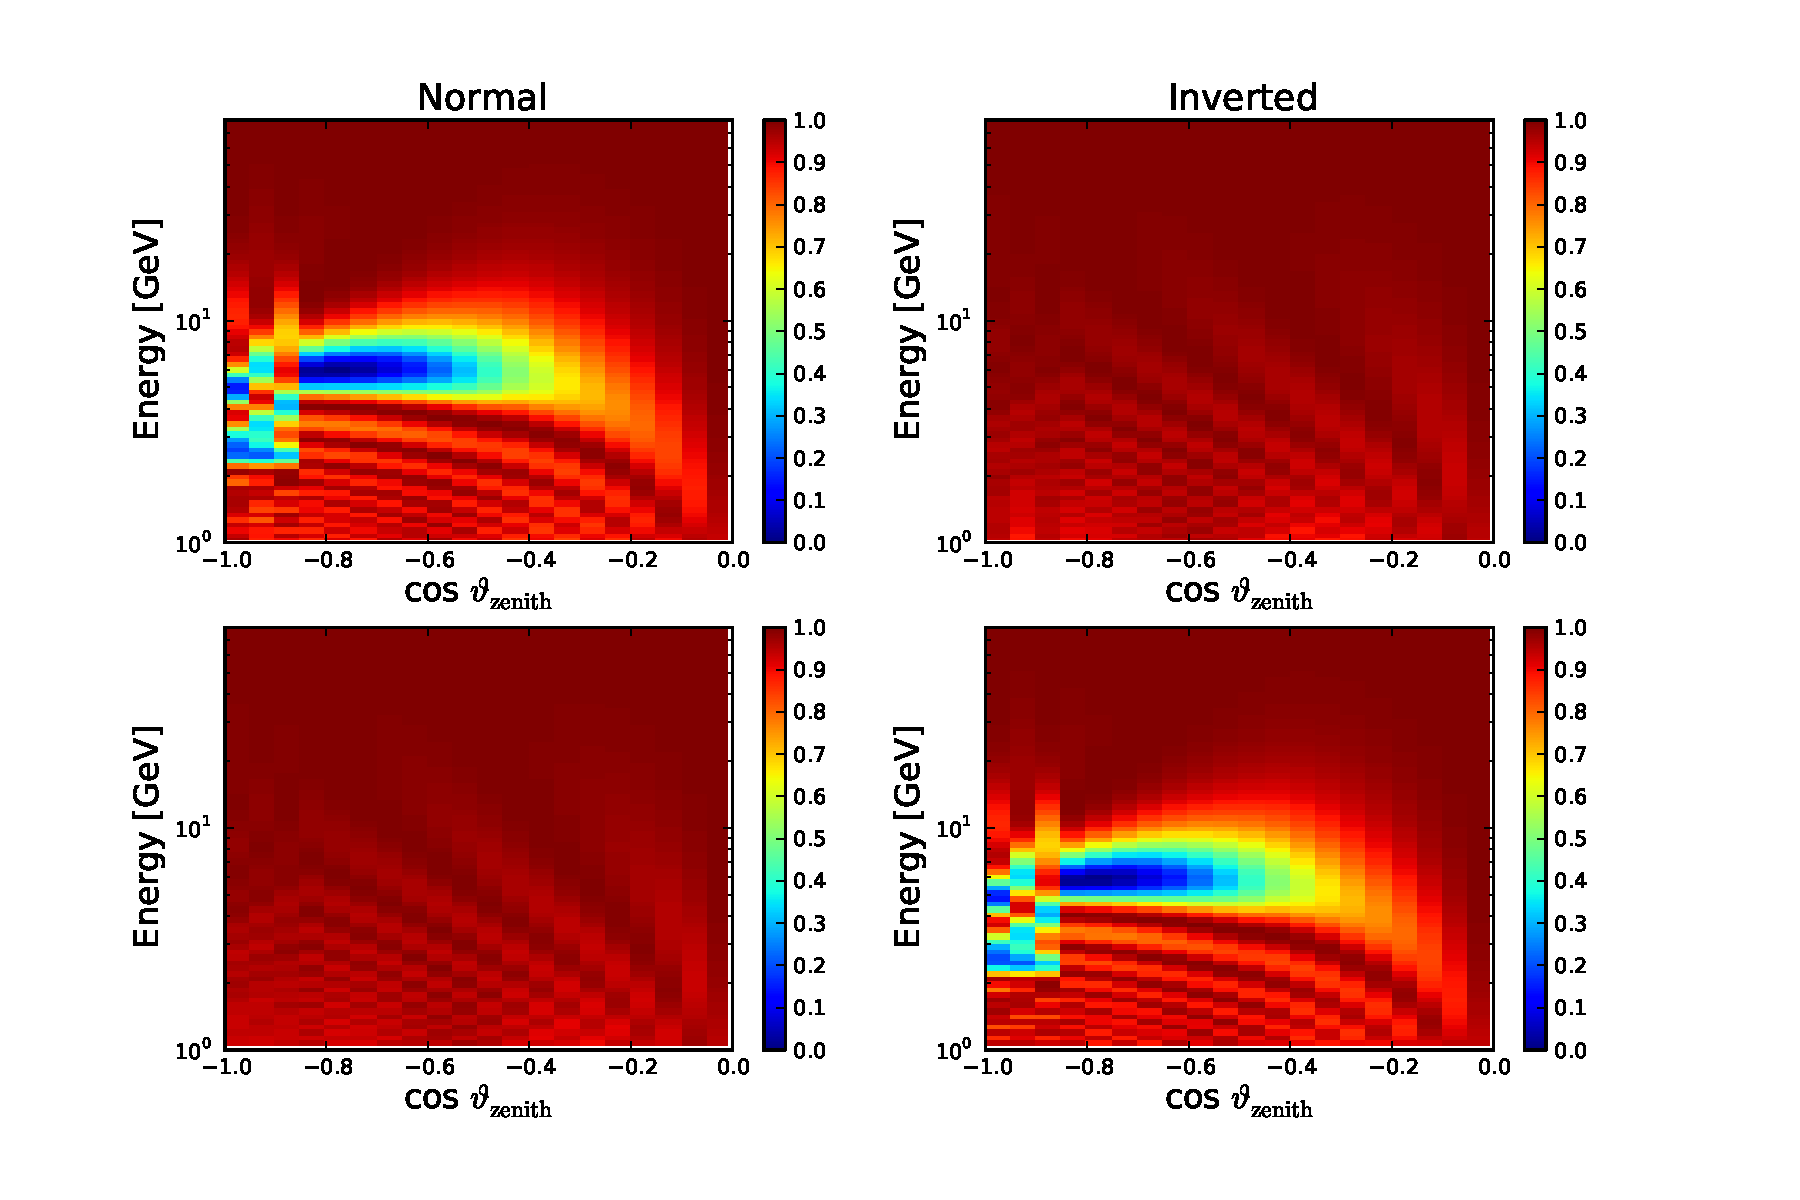
\includegraphics[width=0.95\textwidth]{osc_ds_nue_to_nue}
 \caption{Oscillation probabilities for $\nue \to \nue$ (top) and $\nuebar \to
          \nuebar$ (bottom) for normal and inverted hierarchy.}
\end{figure}


\begin{figure}[t!]
 \centering
 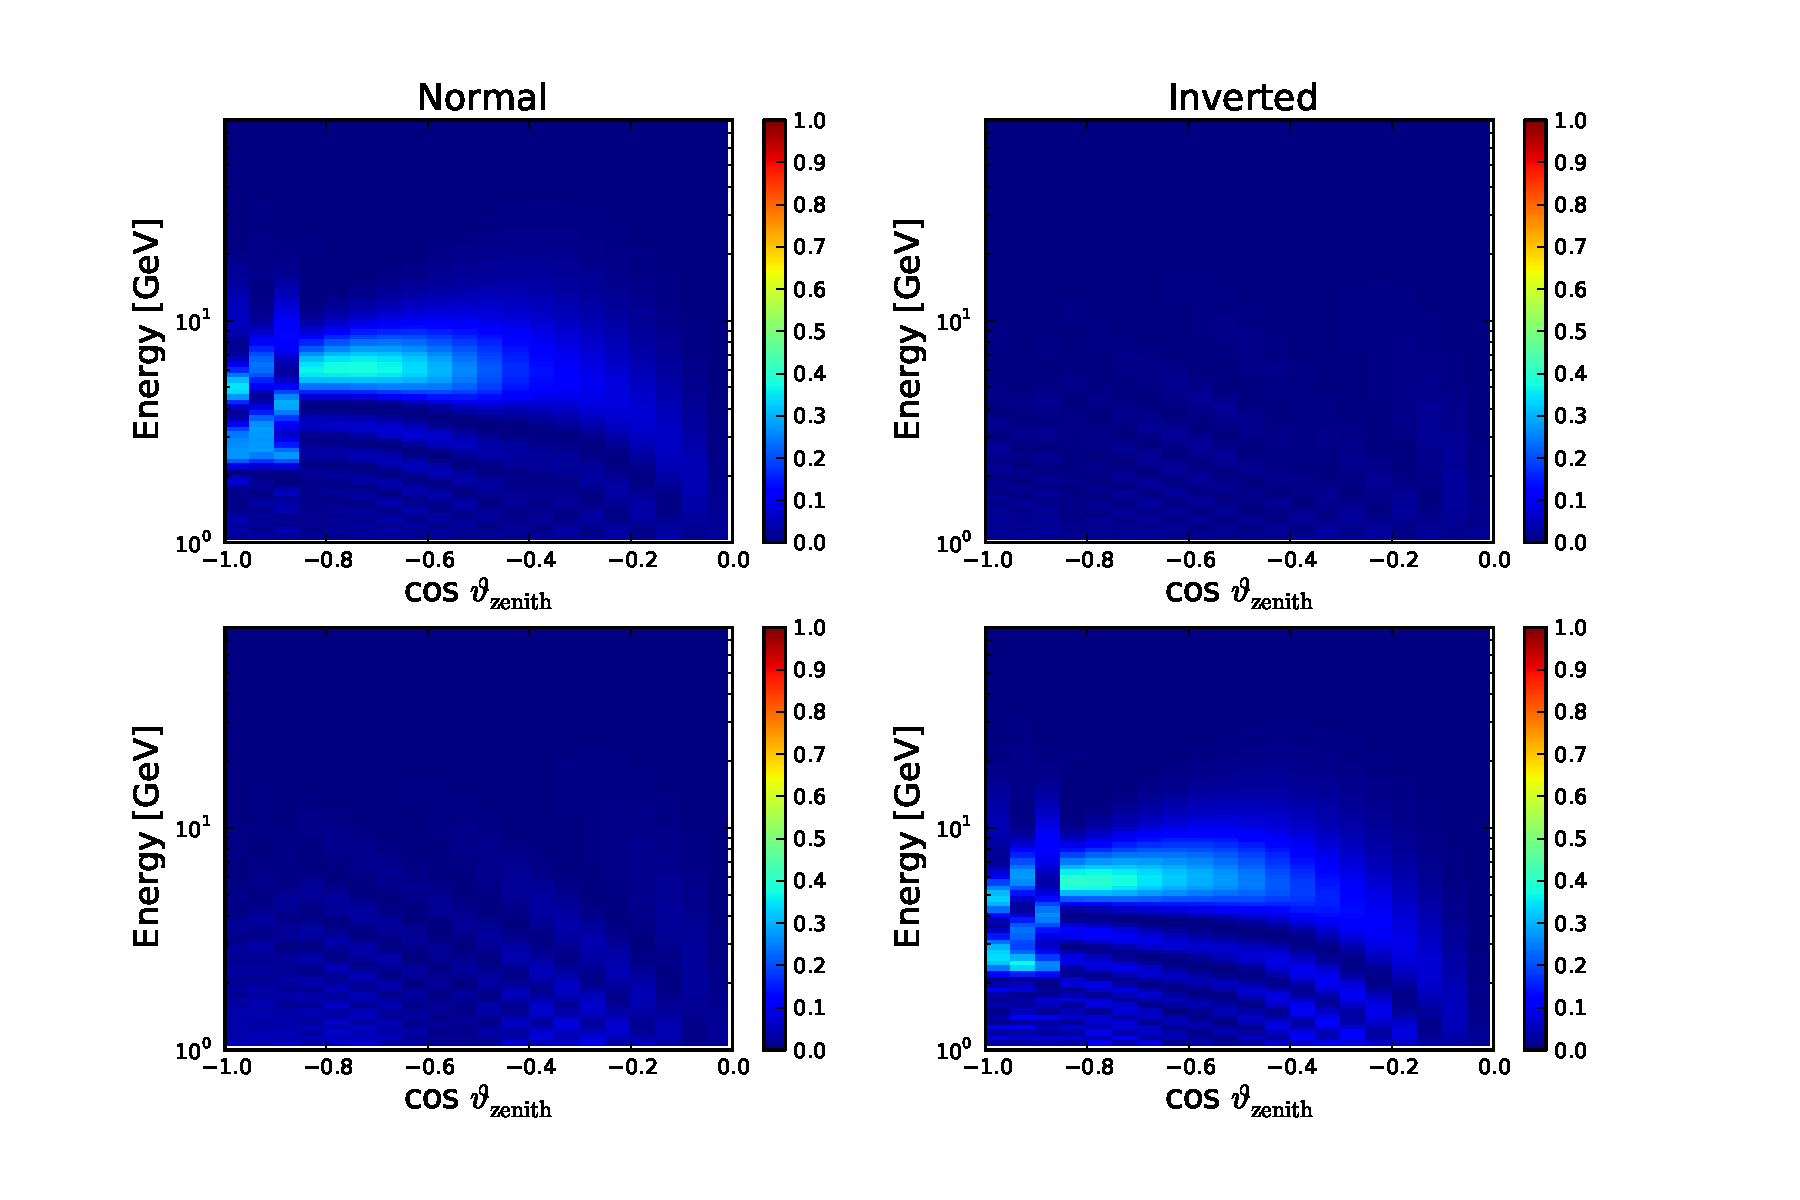
\includegraphics[width=0.95\textwidth]{osc_ds_nue_to_numu}
 \caption{Oscillation probabilities for $\nue \to \numu$ (top) and $\nuebar \to
          \numubar$ (bottom) for normal and inverted hierarchy.}
\end{figure}

\begin{figure}[b!]
 \centering
 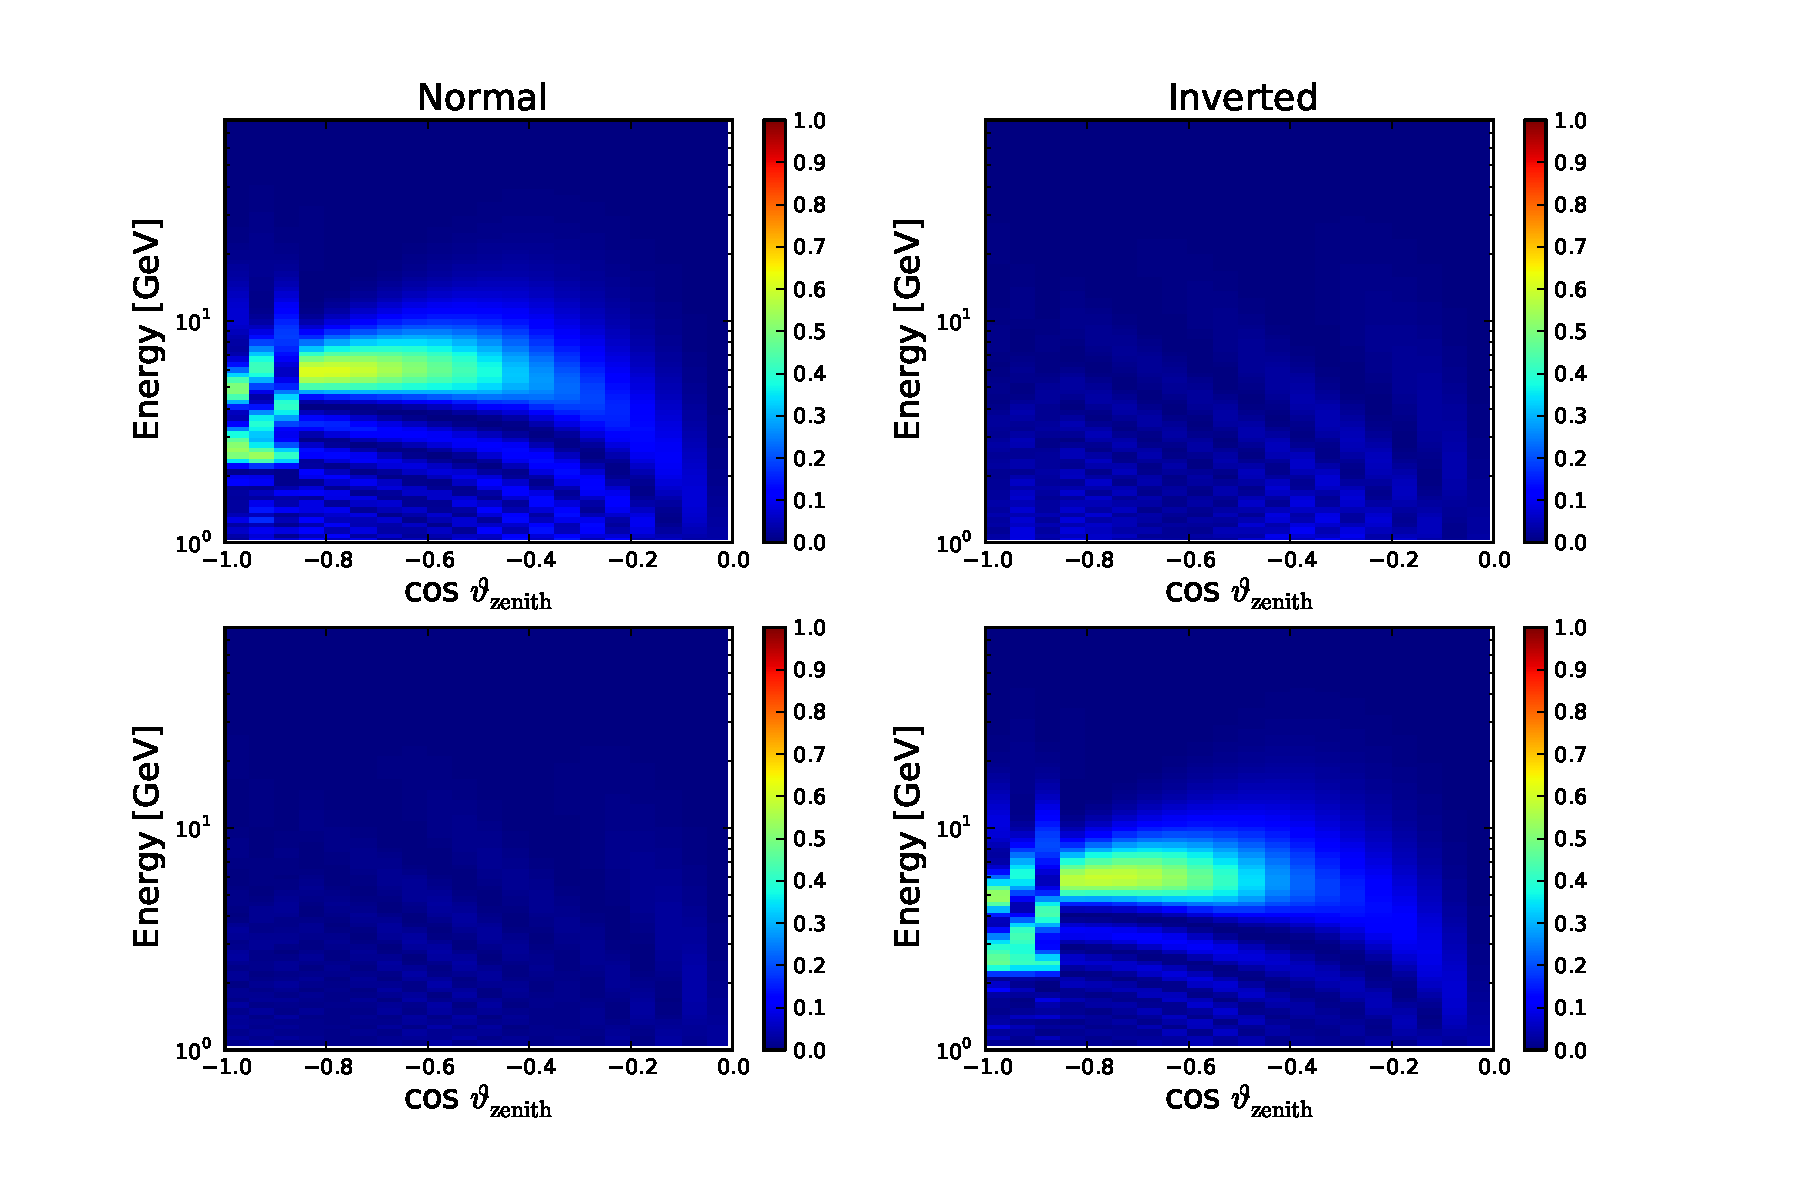
\includegraphics[width=0.95\textwidth]{osc_ds_nue_to_nutau}
 \caption{Oscillation probabilities for $\nue \to \nutau$ (top) and $\nuebar \to
          \nutaubar$ (bottom) for normal and inverted hierarchy.}
\end{figure}

\begin{figure}[t!]
 \centering
 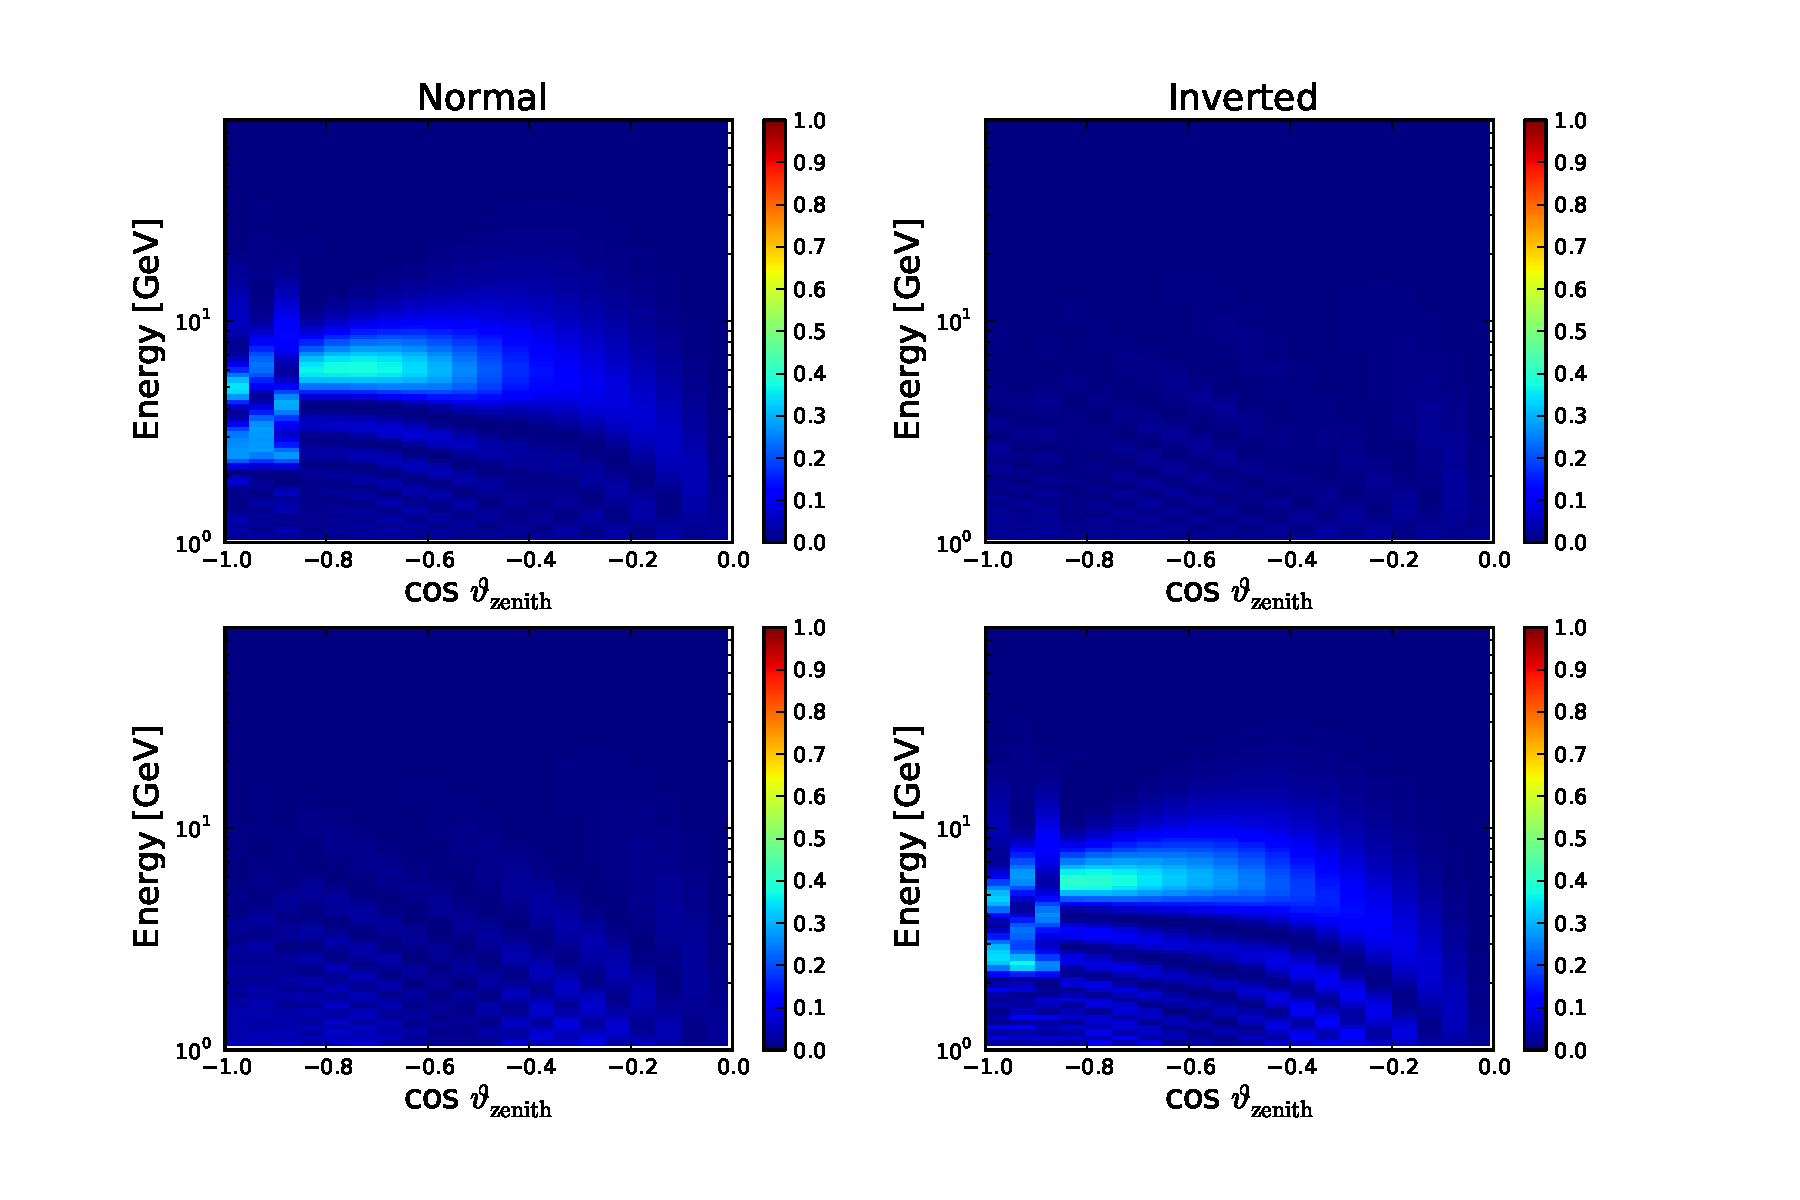
\includegraphics[width=0.95\textwidth]{osc_ds_numu_to_nue}
 \caption{Oscillation probabilities for $\numu \to \nue$ (top) and $\numubar \to
          \nuebar$ (bottom) for normal and inverted hierarchy.}
\end{figure}

\begin{figure}[b!]
 \centering
 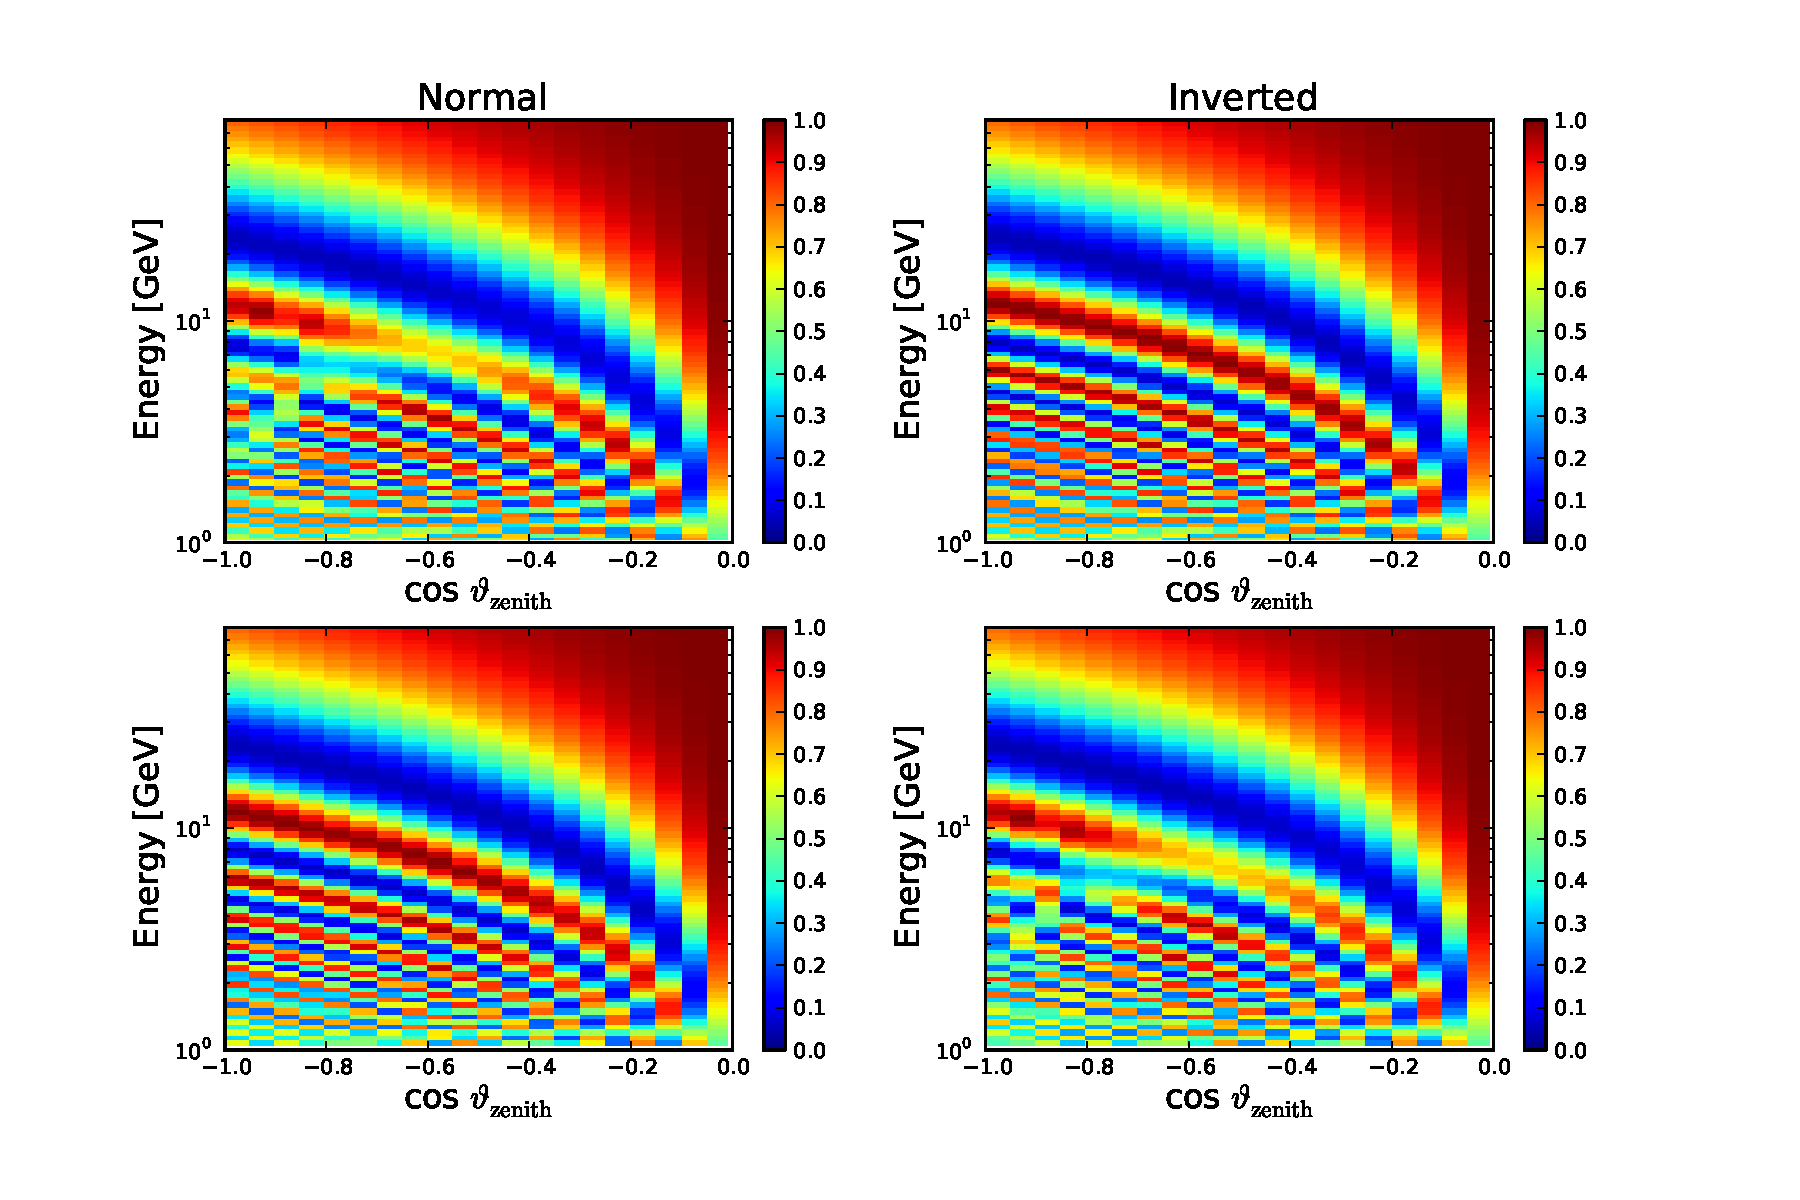
\includegraphics[width=0.95\textwidth]{osc_ds_numu_to_numu}
 \caption{Oscillation probabilities for $\numu \to \numu$ (top) and $\numubar
          \to \numubar$ (bottom) for normal and inverted hierarchy.}
\end{figure}


\begin{figure}[t!]
 \centering
 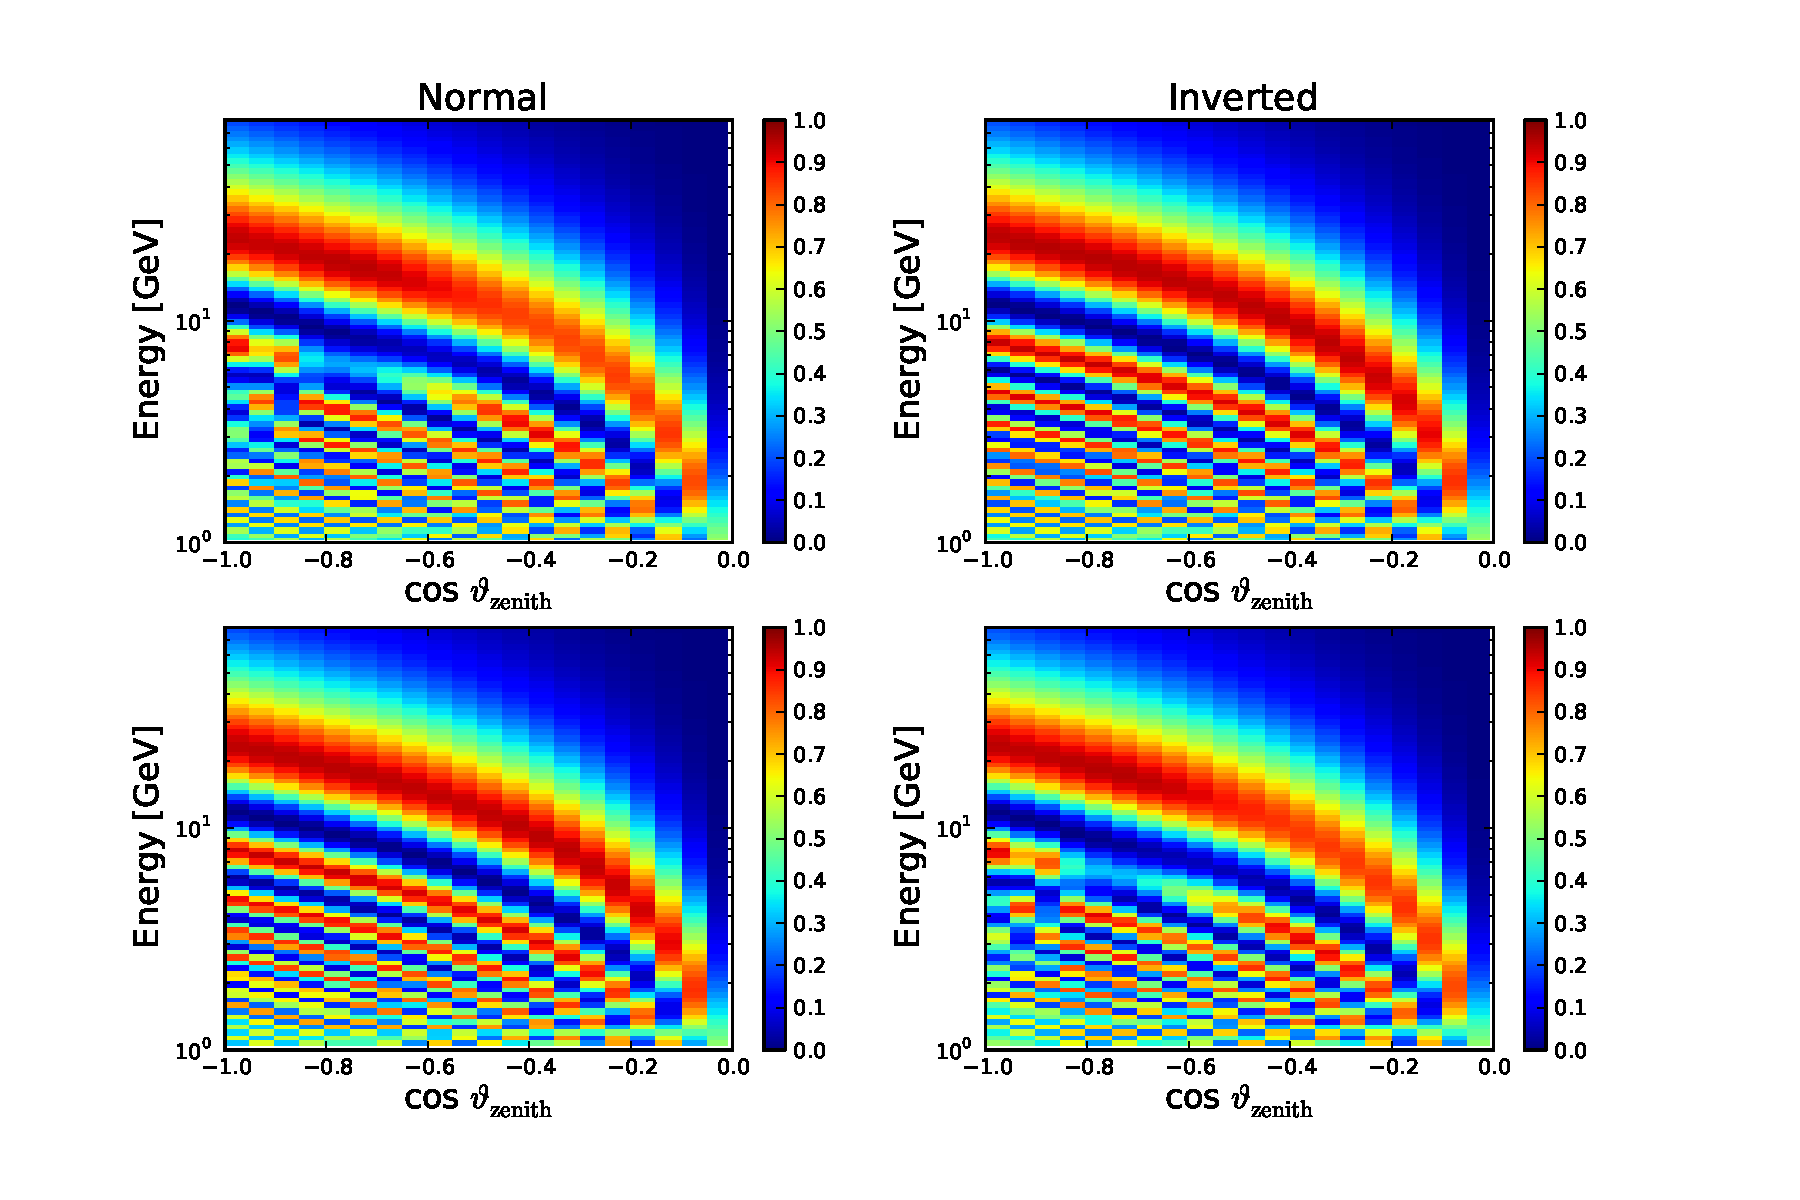
\includegraphics[width=0.95\textwidth]{osc_ds_numu_to_nutau}
 \caption{Oscillation probabilities for $\numu \to \nutau$ (top) and $\numubar
          \to \nutaubar$ (bottom) for normal and inverted hierarchy.}
\end{figure}

\chapter{Parametrisations of the Detector Resolutions}
\label{app:reco_params}

The full parametrisations of the reconstruction performances will be listed in
form of the actual \papa input. These are nested dictionaries giving the
resolutions in energy (\texttt{'e'}) and \coszen (\texttt{'coszen'}) for all
four interaction channels: \nue, \numu, and \nutau CC (\texttt{'nue'},
\texttt{'numu'}, and \texttt{'nutau'}, respectively) and \nux NC
(\texttt{'NC'}). For each of those the resolution is given by the five
parameters \texttt{'fraction'}, \texttt{'loc1'}, \texttt{'loc2'},
\texttt{'width1'}, and \texttt{'width2'}, corresponding to $f$, $\mu_1$,
$\mu_2$, $\sigma_1$ and $\sigma_2$ in (\ref{eqn:reco_param}).

The actual function definitions for the five parameters is then supplied as a
text string that can be interpreted as a python function by python's
\texttt{eval()} function. In those definitions, \texttt{'n'} is a shorthand
for the numpy library \cite{numpy} used for most of the numerical operations in
\papa.

\section{Baseline Settings}

\VerbatimInput{figs/reco_param/reco_default.json}

% \section{Energy Resolution}
% 
% \section{\coszen Resolution}


\chapter{PID Functions}
\label{app:pid}

\section{Baseline Settings}

The particle identification is a binary decision, thus only the track
identification probabilities $P_{\mathrm{channel} \to \mathrm{track}}$ are
listed:
\begin{eqnarray}
 P_{\nue\to\mathrm{track}}(E) =
   0.192 \gauss{\log_{10}(E[\mathrm{GeV}])}{0.878}{0.404} + 0.0309 \\
 P_{\numu\to\mathrm{track}}(E) =
   \frac{0.687}{\stepfunc{\log_{10}(E[\mathrm{GeV}])}{0.683}{0.183}} + 0.0585 \\
 P_{\nutau\to\mathrm{track}}(E) =
   0.197 \gauss{\log_{10}(E[\mathrm{GeV}])}{1.28}{0.466} + 0.0732 \\
 P_{\nux\,\mathrm{NC}\to\mathrm{track}}(E) =
   0.171 \gauss{\log_{10}(E[\mathrm{GeV}])}{1.37}{0.483} + 0.0339
\end{eqnarray}
The cascade identification probabilities are given by $P_{\mathrm{channel} \to
\mathrm{cascade}} = 1 - P_{\mathrm{channel} \to \mathrm{track}}$.